
\section{Ethereum}
Ethereum \cite{buterin2013ethereum} is the second most \href{https://www.crypto51.app/}{secure} public blockchain (\href{https://howmanyconfs.com/}{by about 50\%})\cite{sayeed2019assessing}, and second most valuable by \href{https://coinmarketcap.com/}{market capitalisation} (though this comparison is somewhat stretched). It is the natural connection from Web3 to the rest of the book, so it will be considered first.\par
It is touted as `programmable money'. It, unlike bitcoin, is (\href{https://hackernoon.com/turing-completeness-and-the-ethereum-blockchain-c5a93b865c1a}{nearly}) Turing complete \cite{petzold2008annotated}, able to run a \href{https://ethereum.org/en/developers/docs/evm/}{virtual machine} within the distributed network (albeit slowly), and can therefore process complex transactional contracts in the settlement of value. This has given rise to the new field of `distributed finance', or DeFi (described later), alongside many interesting trust-minimised immutable ledger public database ideas. \par
There are trade-offs and problems with Ethereum (Eth/Ether) which currently increase the `participation floor' and make the network far less suitable for entry level business-to-business use. The ledger itself being a computational engine, with write only properties, is enormous. Specialist cloud hardware is required to run a full node (copy of the ledger), and partial nodes are the norm. Many partial nodes are run by one specialist cloud provider (\href{https://consensys.net/blog/news/why-infura-is-the-secret-weapon-of-ethereum-infrastructure/}{Infura}), which has recently been forced to \href{https://finance.yahoo.com/news/metamask-infura-block-certain-areas-173749914.html}{exclude Venezuela} from the network. Network validators are \href{https://mevwatch.info}{refusing to process} addresses on an \href{https://home.treasury.gov/policy-issues/office-of-foreign-assets-control-sanctions-programs-and-information}{OFAC sanction list}. A staggering 58\% runs on \href{https://ethernodes.org/networkType/Hosting}{Amazon AWS servers}. Critics of the project point to these vulnerabilities to outside influence as an existential threat to the aims of the technology. If it can be censured, then what advantage is there over the \href{https://protos.com/consensys-lawsuit-jpmorgan-owns-critical-ethereum-infrastructure/}{founders} simply running a high speed database to the same purpose? \par
This is a function of the so called `scalability trilema' \cite{hafid2020scaling}, in which it seems that only two features from the list of decentralization, scalability or security can be chosen for blockchains \cite{bonneau2015sok}.\par
Moreover the network is \href{https://bitcoinmagazine.com/technical/ethereum-is-coercive-bitcoin-is-not}{centrally controlled} by its creator and the `miners'. There is a strong case to answer that Eth is \href{https://blog.mollywhite.net/blockchains-are-not-what-they-say/}{neither distributed}, nor trustless, and in fact therefore fails to be differentiated from a DLT, undermining some of it's claims. The history of Ethereum is a fascinating case study in human greed. By the time the whitepaper had it's first limited release, Bitcoin (covered next) had already passed \$1000 per token. This led to the creators ambitions for a `fair release' of tokens being voted down by powerful funders, leading to the explosion of similarly structured `pre-mined' coins in the ICO craze, which followed on the Ethereum network. Laura Shin is possibly the most experienced journalist and author in the space and has covered this crazy era in her book `The Cryptopians' \cite{cryptopians}. It's a tough read for the newcomer though, perhaps finish this primer first!\par
With that said there are many talented developers doing interesting work on the platform, and innovation is fast paced. It is entirely normal for technology projects to launch their distributed ledger idea on and within the Ethereum network. These generate tradable `ERC-20' tokens, which can accrue value or demonstrate smart contract utility  (based on the \href{https://soliditylang.org/}{Solidity} programming language). Because the value locked and generated in the Ethereum platform comes not just from the ETH token, but all the ERC technologies built upon it, there are hundreds of billions of pounds `within' the network. All of these projects, and indeed the core technology of Ethereum are subject to exploits and vulnerabilities and tens of billions of pounds have been lost \cite{chen2020survey}. Most of this money is pure market speculation (as is the case across blockchains). Many analysts cannot see this as anything but a speculative bubble, with all the predictable crash yet to come. This can be seen in the context of other bubbles in Figure \ref{fig:etherbubble}. It seems that most of the projects in crypto more generally, but certainly with ETH and the NFTs within it are a new kind of social gambling, where online communities can reinforce groupthink around their speculative choices. This idea that Ethereum is not a commodity, but rather a security, built around promises of returns, is finding recent favour in law. New York attorney general James has alleged that Ether is a security in \href{https://www.docdroid.net/Myyp0yz/kucoin-pdf#page=11}{court proceedings}, which could have enormous consequences, potentially reversing the momentum the asset had been enjoying as a commodity.   Jason Lowery of MIT and US Space Force \href{https://twitter.com/JasonPLowery/status/1572275617344757760}{lays out} a very clear thesis on the difference between Natamoto consensus and most of what followed as part of his PhD \cite{Lowery2023}. His explanation here is proximal to why we focus on Bitcoin, and dismiss `proof of stake' models, though Lowery himself has very serious detractors such as Voskuil who has been working on these problems for a long time \cite{voskuil2020cryptoeconomics} \par
it{``The innovation behind PoW is precisely the fact that it \textbf{doesn't} rely exclusively on software (an abstraction) to keep the ledger systemically secure, but instead incorporates real-world physics (watts) to impose real-world physical constraints on people/computers who run it. Stake is an abstraction. It is an imaginary way to describe the complex emergent behaviour of a bunch of general-purpose state machines. The state machines may physically exist, but the way you choose to visualize the complex emergent behaviour of those machines is imaginary. Satoshi didn't couple control authority over ledger to abstract, imaginary things like `stake' or `coin' precisely because these things don't physically exist. If they don't physically exist, they are incapable of imposing real-world physical costs on people seeking control of ledger. The real-world physical cost of controlling the ledger is what keeps control over the ledger decentralized. It is too physically expensive (in watts) to gain and maintain centralized control over the BTC ledger. In proof of stake, there is no physical cost of gaining centralized control. Why? Because stake doesn't physically exist. So all it takes to gain centralized control is majority stake. And once you have it (which, because of math, some combination of people already do), you have it forever.}


With all this said most of the \href{https://www.statista.com/statistics/1266322/nft-user-number/}{couple of million people} who have used NFTs use Ethereum, and if this market of creators and consumers is to be brought into a mixed reality space then they will need a way to bring their objects with them. 
\begin{figure}
  \centering
    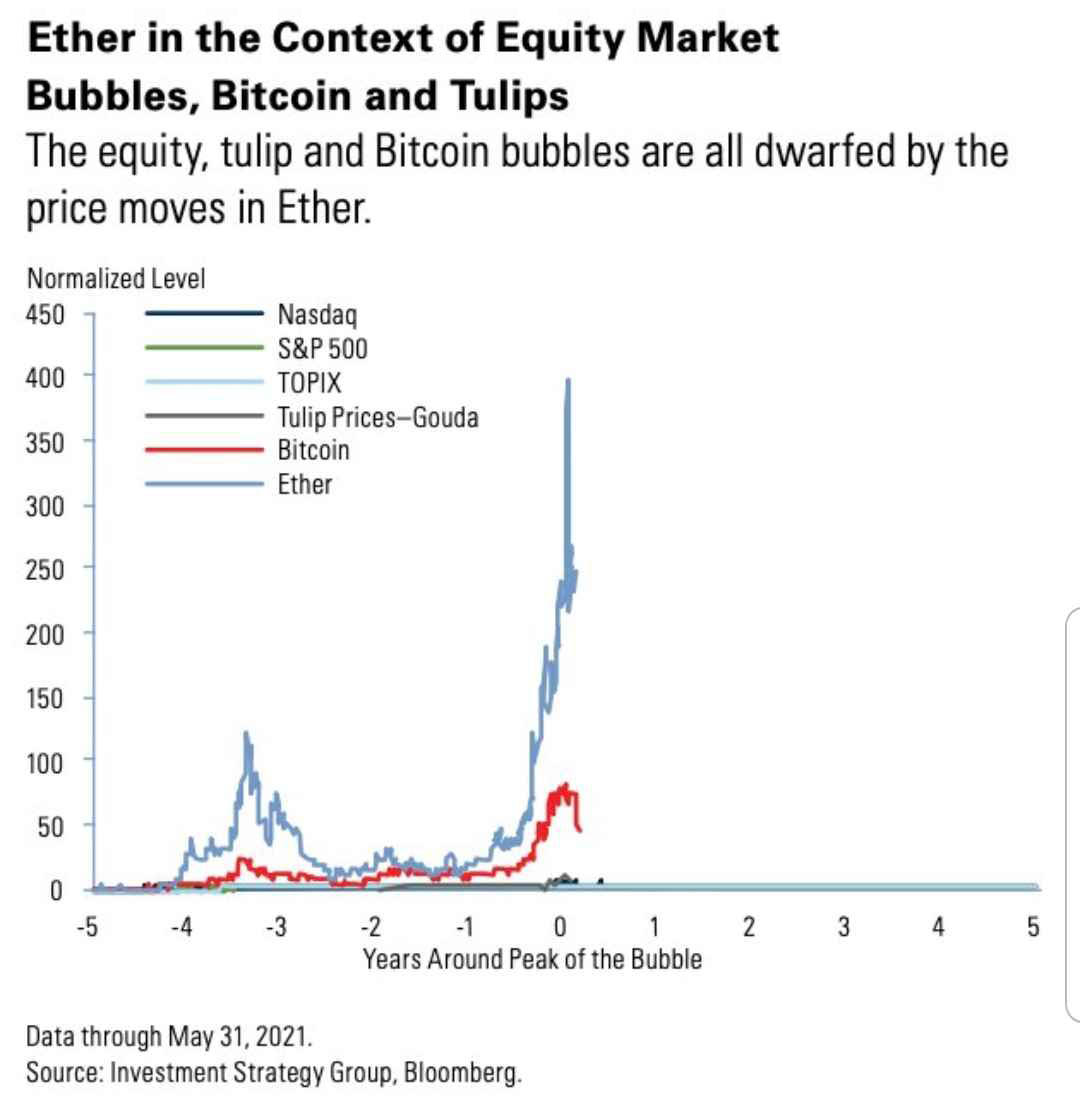
\includegraphics{etherbubble}
  \caption{Ethereum is thought to look like a speculative bubble. Rights requested}
    \label{fig:etherbubble}
\end{figure}
Such is the level of nefarious activity on these networks (within Ethereum) that they have a poor reputation, and are difficult to audit, launch, and maintain. The overriding problem of using a blockchain for utility applications (rather than just as money) is that people can, and will, simply lie for criminal purpose when entering data into the ledger. It is far more likely that Ethereum is simply a speculative bubble than any of the claims for utility being born out. Add to that \href{https://advisor.morganstanley.com/daron.edwards/documents/field/d/da/daron-edwards/Cryptocurrency_201__What_is_Ethereum_.pdf}{Morgan Stanleys recent assertion} that Ethereum is itself threatened by newer contender chains and it's future becomes unclear. The report correctly identifies that ``High transaction fees create scalability problems and threaten user demand. High costs make Ethereum too expensive for small-value transactions.''. It is this high cost of use that most excludes the ERC-20 networks from our consideration.
\subsection{Gas fees}
Ethereum has a significant barrier to entry because of high fees to use the network. The system is Turing complete; able to programatically replicate any other computational system. This includes endless loops in code, so it is trivial to lock up the computational bandwidth of the whole system, in a smart contract commitment, through a web wallet. \par 
To mitigate this existential `denial of service attack' the `gas' system demands that users spend some of their locked up value to operate on the network. In this way a transaction loop would quickly erode the available gas and stop looping. As the popularity of the system has grown, so too have the gas fees. It can \href{https://twitter.com/Blockworks_/status/1521071340517830657}{sometimes cost} over £10,000 to do a single transaction, though it is typically a few tens of pounds. Appallingly if the user pitches their mining fee offer too low, then the money gets spent anyway! \href{https://fees.wtf/#/}{A website} just plucks random Ethereum addresses out of the aether to show you the level of this expense for participants. People can even \href{https://opensea.io/collection/fees-wtf-nft?search[sortAscending]=false&search[sortBy]=PRICE}{buy NFTs} of the worst examples of these, as `tokens', wasting more money. This is a huge problem for potential uses of the network. \par
\subsection{Ether ultra hard money narrative}
Part of the challenge Ethereum faces is wrapped up with it's complex token emission schedule. This is the rate at which tokens are generated and `burnt' or destroyed in the network. The total supply of tokens is uncertain, and both emission and burn schedules are regularly tinkered with by the project. The changes to the rate at which ETH are generated can be seen in Figure \ref{fig:ethemission}.
\begin{figure}
  \centering
    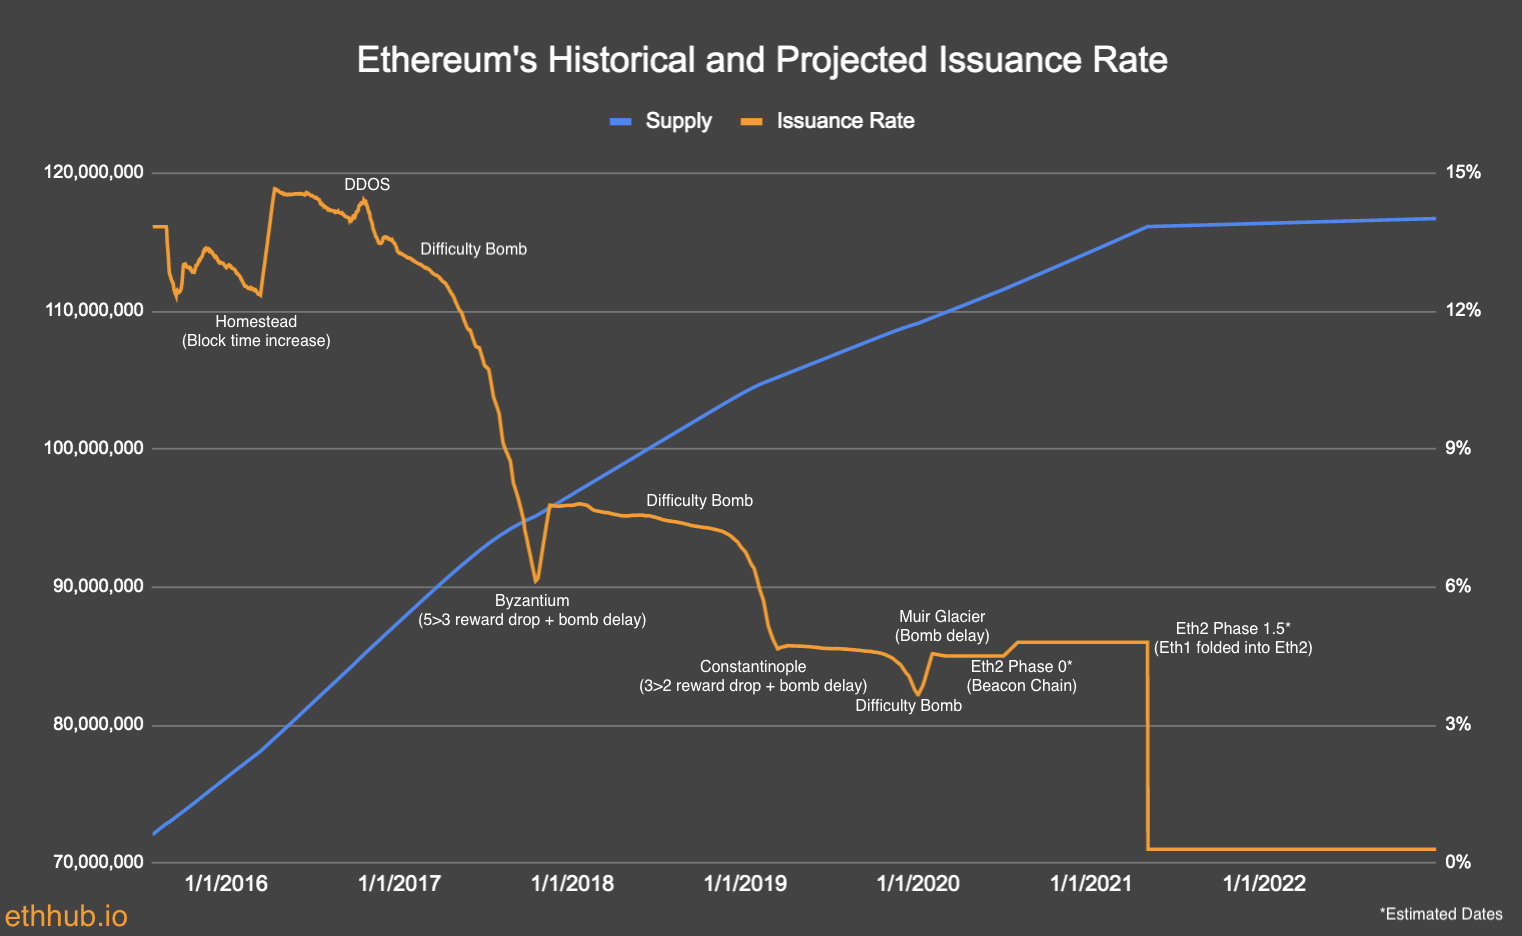
\includegraphics{ethemission}
  \caption{The rate of token generation has changed unpredictably over time. Rights requested}
  \label{fig:ethemission}
\end{figure}
In addition, a recent upgrade (EIP-1559) results in tokens now being burnt at a higher rate than they are produced, deliberately leading to a diminishing supply. In theory this increases the value of each ETH on the network at around 1\% per year. It's very complex, with impacts on transaction fees, waiting time, and consensus security, as examined by Liu at al. \cite{liu2022empirical}. Additionally, there is now talk (by \href{https://time.com/6158182/vitalik-buterin-ethereum-profile/}{Butlerin}, the creator of Ethereum) of extending this burn mechanism \href{https://ethresear.ch/t/multidimensional-eip-1559/11651}{further into the network}.\par
Ethereum was designed from the beginning to move to a `proof of stake' model where token holders underpin network consensus through complex automated voting systems based upon their token holding. This is now called \href{https://blog.ethereum.org/2022/01/24/the-great-eth2-renaming/}{Ethereum Consensus Layer}.  This recent `Merge' upgrade has reduced the carbon footprint of the network, a laudable thing, though it seems the GPUs and datacentres have just gone on to be elsewhere. It has not lowered the cost to users nor improved performance. As part of the switching roadmap users were asked to lock up 32ETH tokens each (a substantial allocation of capital). In total there are around 14 million of these tokens, and it is those users who now control the network. This money is likely stuck on the network until at least 2024, a significant delay wen compared to the original promises.\par
This means that proof of stake has problems in that the majority owners `decide' the truth of the chain to a degree, and must by design have the ability to over-ride prior consensus choices. Remember that these users are now trapped in their positions. Four major entities now control the rules of the chain, and have already agreed to censor certain banned addressees. Proof of stake is probably inherently broken \cite{poelstra2015stake}. This has \href{https://notes.ethereum.org/@djrtwo/risks-of-lsd} for malicious actors who have sufficient control of the existing history of the chain, \href{https://twitter.com/MTorgin/status/1521433474820890624}{thought to be} in the region of \$50M \cite{mackinga2022twap}. Like much of the rest of `crypto' the proposed changes will concentrate decisions and economic rewards in the hands of major players, early investors, and incumbents. This is a far cry from the stated aims of the technology. The move to proof of stake has recently earned it the \href{https://www.technologyreview.com/2022/02/23/1044960/proof-of-stake-cryptocurrency/}{MIT breakthrough technology award}, despite not being complete (validators cannot yet sell their voting stakes). It's clearly a technology which is designed to innovate at the expense of predictability. This might work out very well for the platform, but right now the barrier to participation (in gas fees) is so high that we do not intend for Ethereum to be in scope as a method for value transfer within metaverses.\par
%\subsubsection{Consequences of hard forks}
%Ethereums strategy has been that of uncontentious \href{https://ethereum.org/en/history/}{``canonical hard forks''}. These regular changes to the distributed codebase are well managed so as to not result in bifurcations of the network such as the \href{https://www.gemini.com/cryptopedia/ethereum-classic-etc-vs-eth}{Ethereum Classic fork}. In a contentious hard fork two different versions of the chain move forward with different incentives and design choices. This could conceivable happen in the switch to POS, and indeed there are some signs that Ethereum miners are already gearing up to move back to supporting ``classic'' which will be a \href{https://fortune.com/2022/07/29/eth-price-ethereum-original-coin-soar-miners-migrate-ahead-of-merge/}{huge boon to the legacy fork}. If there is another contentious split at ``The Merge'' point, with a cabal of miners supporting the current system and trying to remove the \href{https://ethereum.org/en/glossary/#difficulty-bomb}{difficulty bomb} which is supposed to \href{https://gitter.im/ethereum/AllCoreDevs?at=5dd4f6bfe5ea5550f4db3d78}{clean this problem up}, then there will suddenly exist 2 copies of every NFT and asset on the chain. This is unlikely as it would require some buy in from nodes and users, but an under discussed risk to the system. Were it to happen many people would choose the wrong chain and sell the asset on the wrong side of the bet.
\subsection{Inherent Weaknesses}
Ethereum faces a unique dilemma, often overshadowed by its technological capabilities. Unlike Bitcoin (BTC), which has solidified its role as a stable and reliable store of value, Ethereum's value proposition is more complex and, ultimately, paradoxical. The following points elaborate on this conundrum:

\begin{itemize}
    \item \textbf{Lack of Monetary Certainty:} Ethereum's mutable supply schedule and governance model introduce a level of uncertainty not found in Bitcoin. 
    \item \textbf{Equity-like Characteristics:} Ethereum acts more like a share in a semi-decentralized corporation than a straightforward asset, deriving its value from expected future transaction fees.
\end{itemize}

These attributes lead to a value paradox that is two-fold:

\begin{itemize}
    \item \textbf{Fee Dilemma:} High transaction fees, while beneficial for Ethereum's perceived value, deter usage and drive decentralized finance (DeFi) applications to other platforms.
    \item \textbf{Scalability Trap:} Attempts to scale the platform and lower fees would, counterintuitively, reduce Ethereum's intrinsic value by decreasing its future cash flows.
\end{itemize}

This presents a catch-22 situation where Ethereum's value is fundamentally limited by its own economic model. If the asset's value drops significantly, it could undermine the security of the entire platform, making it less reliable for settling large transactions.

In the long run, this creates a feedback loop that could, theoretically, push Ethereum's value towards zero. This issue casts a shadow over Ethereum's long-term viability, presenting a challenge that goes beyond mere technical scalability.
